% Options for packages loaded elsewhere
\PassOptionsToPackage{unicode}{hyperref}
\PassOptionsToPackage{hyphens}{url}
%
\documentclass[
]{article}
\usepackage{amsmath,amssymb}
\usepackage{iftex}
\ifPDFTeX
  \usepackage[T1]{fontenc}
  \usepackage[utf8]{inputenc}
  \usepackage{textcomp} % provide euro and other symbols
\else % if luatex or xetex
  \usepackage{unicode-math} % this also loads fontspec
  \defaultfontfeatures{Scale=MatchLowercase}
  \defaultfontfeatures[\rmfamily]{Ligatures=TeX,Scale=1}
\fi
\usepackage{lmodern}
\ifPDFTeX\else
  % xetex/luatex font selection
\fi
% Use upquote if available, for straight quotes in verbatim environments
\IfFileExists{upquote.sty}{\usepackage{upquote}}{}
\IfFileExists{microtype.sty}{% use microtype if available
  \usepackage[]{microtype}
  \UseMicrotypeSet[protrusion]{basicmath} % disable protrusion for tt fonts
}{}
\makeatletter
\@ifundefined{KOMAClassName}{% if non-KOMA class
  \IfFileExists{parskip.sty}{%
    \usepackage{parskip}
  }{% else
    \setlength{\parindent}{0pt}
    \setlength{\parskip}{6pt plus 2pt minus 1pt}}
}{% if KOMA class
  \KOMAoptions{parskip=half}}
\makeatother
\usepackage{xcolor}
\usepackage[margin=1in]{geometry}
\usepackage{color}
\usepackage{fancyvrb}
\newcommand{\VerbBar}{|}
\newcommand{\VERB}{\Verb[commandchars=\\\{\}]}
\DefineVerbatimEnvironment{Highlighting}{Verbatim}{commandchars=\\\{\}}
% Add ',fontsize=\small' for more characters per line
\usepackage{framed}
\definecolor{shadecolor}{RGB}{248,248,248}
\newenvironment{Shaded}{\begin{snugshade}}{\end{snugshade}}
\newcommand{\AlertTok}[1]{\textcolor[rgb]{0.94,0.16,0.16}{#1}}
\newcommand{\AnnotationTok}[1]{\textcolor[rgb]{0.56,0.35,0.01}{\textbf{\textit{#1}}}}
\newcommand{\AttributeTok}[1]{\textcolor[rgb]{0.13,0.29,0.53}{#1}}
\newcommand{\BaseNTok}[1]{\textcolor[rgb]{0.00,0.00,0.81}{#1}}
\newcommand{\BuiltInTok}[1]{#1}
\newcommand{\CharTok}[1]{\textcolor[rgb]{0.31,0.60,0.02}{#1}}
\newcommand{\CommentTok}[1]{\textcolor[rgb]{0.56,0.35,0.01}{\textit{#1}}}
\newcommand{\CommentVarTok}[1]{\textcolor[rgb]{0.56,0.35,0.01}{\textbf{\textit{#1}}}}
\newcommand{\ConstantTok}[1]{\textcolor[rgb]{0.56,0.35,0.01}{#1}}
\newcommand{\ControlFlowTok}[1]{\textcolor[rgb]{0.13,0.29,0.53}{\textbf{#1}}}
\newcommand{\DataTypeTok}[1]{\textcolor[rgb]{0.13,0.29,0.53}{#1}}
\newcommand{\DecValTok}[1]{\textcolor[rgb]{0.00,0.00,0.81}{#1}}
\newcommand{\DocumentationTok}[1]{\textcolor[rgb]{0.56,0.35,0.01}{\textbf{\textit{#1}}}}
\newcommand{\ErrorTok}[1]{\textcolor[rgb]{0.64,0.00,0.00}{\textbf{#1}}}
\newcommand{\ExtensionTok}[1]{#1}
\newcommand{\FloatTok}[1]{\textcolor[rgb]{0.00,0.00,0.81}{#1}}
\newcommand{\FunctionTok}[1]{\textcolor[rgb]{0.13,0.29,0.53}{\textbf{#1}}}
\newcommand{\ImportTok}[1]{#1}
\newcommand{\InformationTok}[1]{\textcolor[rgb]{0.56,0.35,0.01}{\textbf{\textit{#1}}}}
\newcommand{\KeywordTok}[1]{\textcolor[rgb]{0.13,0.29,0.53}{\textbf{#1}}}
\newcommand{\NormalTok}[1]{#1}
\newcommand{\OperatorTok}[1]{\textcolor[rgb]{0.81,0.36,0.00}{\textbf{#1}}}
\newcommand{\OtherTok}[1]{\textcolor[rgb]{0.56,0.35,0.01}{#1}}
\newcommand{\PreprocessorTok}[1]{\textcolor[rgb]{0.56,0.35,0.01}{\textit{#1}}}
\newcommand{\RegionMarkerTok}[1]{#1}
\newcommand{\SpecialCharTok}[1]{\textcolor[rgb]{0.81,0.36,0.00}{\textbf{#1}}}
\newcommand{\SpecialStringTok}[1]{\textcolor[rgb]{0.31,0.60,0.02}{#1}}
\newcommand{\StringTok}[1]{\textcolor[rgb]{0.31,0.60,0.02}{#1}}
\newcommand{\VariableTok}[1]{\textcolor[rgb]{0.00,0.00,0.00}{#1}}
\newcommand{\VerbatimStringTok}[1]{\textcolor[rgb]{0.31,0.60,0.02}{#1}}
\newcommand{\WarningTok}[1]{\textcolor[rgb]{0.56,0.35,0.01}{\textbf{\textit{#1}}}}
\usepackage{graphicx}
\makeatletter
\def\maxwidth{\ifdim\Gin@nat@width>\linewidth\linewidth\else\Gin@nat@width\fi}
\def\maxheight{\ifdim\Gin@nat@height>\textheight\textheight\else\Gin@nat@height\fi}
\makeatother
% Scale images if necessary, so that they will not overflow the page
% margins by default, and it is still possible to overwrite the defaults
% using explicit options in \includegraphics[width, height, ...]{}
\setkeys{Gin}{width=\maxwidth,height=\maxheight,keepaspectratio}
% Set default figure placement to htbp
\makeatletter
\def\fps@figure{htbp}
\makeatother
\setlength{\emergencystretch}{3em} % prevent overfull lines
\providecommand{\tightlist}{%
  \setlength{\itemsep}{0pt}\setlength{\parskip}{0pt}}
\setcounter{secnumdepth}{-\maxdimen} % remove section numbering
\usepackage{booktabs}
\usepackage{caption}
\usepackage{longtable}
\usepackage{colortbl}
\usepackage{array}
\ifLuaTeX
  \usepackage{selnolig}  % disable illegal ligatures
\fi
\IfFileExists{bookmark.sty}{\usepackage{bookmark}}{\usepackage{hyperref}}
\IfFileExists{xurl.sty}{\usepackage{xurl}}{} % add URL line breaks if available
\urlstyle{same}
\hypersetup{
  pdftitle={lakewatch lake template batch processing},
  hidelinks,
  pdfcreator={LaTeX via pandoc}}

\title{lakewatch lake template batch processing}
\author{}
\date{\vspace{-2.5em}}

\begin{document}
\maketitle

\begin{Shaded}
\begin{Highlighting}[]
\CommentTok{\#tinytex::tlmgr\_update()}
\end{Highlighting}
\end{Shaded}

\hypertarget{florida-lakewatch-report-for-lake-in-county-county-using-data-downloaded-1292022}{%
\subsection{Florida LAKEWATCH Report for «Lake» in «County» County Using
Data Downloaded
12/9/2022}\label{florida-lakewatch-report-for-lake-in-county-county-using-data-downloaded-1292022}}

\hypertarget{introduction-for-lakes}{%
\subsubsection{Introduction for Lakes}\label{introduction-for-lakes}}

This report summarizes data collected on systems that have been part of
the LAKEWATCH program. Data are from the period of record for individual
systems. Part one allows the comparison of data with Florida Department
of Environmental Protection's Numeric Nutrient Criteria. Part two allows
a comparison of the long-term mean nutrient concentrations with nutrient
zone concentrations published by LAKEWATCH staff (Bachmann et al.~2012;
\url{https://lakewatch.ifas.ufl.edu/resources/bibliography/}). Finally,
this report examines data for long-term trends that may be occurring in
individual systems but only for systems with \textbf{five or more years
of data}. Step by step instructions on how to use the data tables are
provided on page 4 of this report.

\hypertarget{florida-department-of-environmental-protection-fdep-nutrient-criteria-for-lakes-table-1}{%
\subsubsection{Florida Department of Environmental Protection (FDEP)
Nutrient Criteria for Lakes (Table
1)}\label{florida-department-of-environmental-protection-fdep-nutrient-criteria-for-lakes-table-1}}

For lakes, the numeric interpretations of the nutrient criterion in
paragraph 62-302.530(47)(b), F.A.C., based on chlorophyll are shown in
Table 1. The applicable interpretations for TN and TP will vary on an
annual basis, depending on the availability and concentration of
chlorophyll data for the lake. The numeric interpretations for TN, TP,
and chlorophyll shall not be exceeded more than once in any consecutive
three year period.

\begin{enumerate}
\def\labelenumi{\alph{enumi}.}
\item
  If annual geometric mean chlorophyll does not exceed the chlorophyll
  value for one of three lake classification groups listed in the table
  below, then the TN and TP numeric interpretations for that calendar
  year shall be the annual geometric means of the maximum calculated
  numeric interpretation in Table 1.
\item
  If there are insufficient data to calculate the annual geometric mean
  chlorophyll for a given year or the annual geometric mean chlorophyll
  exceeds the values in Table 1 for the correct lake classification
  group, then the applicable numeric interpretations for TN and TP shall
  be the minimum values in Table 1.
\end{enumerate}

\hypertarget{long-term-data-summary-for-lakes-table-2-definitions}{%
\subsubsection{Long-Term Data Summary for Lakes (Table 2):
Definitions}\label{long-term-data-summary-for-lakes-table-2-definitions}}

\begin{itemize}
\tightlist
\item
  \textbf{Total Phosphorus (µg/L):} Nutrient most often limiting growth
  of plant/algae.
\item
  \textbf{Total Nitrogen (µg/L):} Nutrient needed for aquatic
  plant/algae growth but only limiting when nitrogen to phosphorus
  ratios are generally less than 10 (by mass).
\item
  \textbf{Chlorophyll-uncorrected (µg/L):} Chlorophyll concentrations
  are used to measure relative abundances of open water algae.
\item
  \textbf{Secchi (ft), Secchi (m):} Secchi measurements are estimates of
  water clarity.
\item
  \textbf{Color (Pt-Co Units):} LAKEWATCH measures true color, which is
  the color of the water after particles have been filtered out.
\item
  \textbf{Specific Conductance (µS/cm @ 25 C):} Measurement of the
  ability of water to conduct electricity and can be used to estimate
  the amount of dissolved materials in water.
\item
  \textbf{Lake Classification:} Numeric nutrient criteria for Florida
  require that lakes must first be classified into one of three group
  based on color and alkalinity or specific conductance; \textbf{colored
  lakes} (color greater than 40 Pt-Co units), \textbf{clear soft water
  lakes} (color less than or equal to 40 Pt-Co units and alkalinity less
  than or equal to 20 mg/L as CaCO3 or specific conductance less than or
  equal to 100 µs/cm @25 C), and \textbf{clear hard water lakes} (color
  less than 40 Pt-Co units and alkalinity greater than 20 mg/L as CaCO3
  or specific conductance greater 100 µS/cm @ 25 C).
\end{itemize}

\hypertarget{table-1.-florida-department-of-environmental-protections-numeric-nutrient-criteria-for-lakes.}{%
\subsubsection{Table 1. Florida Department of Environmental Protection's
Numeric Nutrient Criteria for
lakes.}\label{table-1.-florida-department-of-environmental-protections-numeric-nutrient-criteria-for-lakes.}}

{[}1 For lakes with color \textgreater{} 40 PCU in the West Central
Nutrient Watershed Region, the maximum TP limit shall be the 490 µg/L TP
streams threshold for the region.{]}

\begin{Shaded}
\begin{Highlighting}[]
\NormalTok{knitr}\SpecialCharTok{::}\FunctionTok{include\_graphics}\NormalTok{(}\StringTok{"LW Reports Table 1 V.2.png"}\NormalTok{)}
\end{Highlighting}
\end{Shaded}

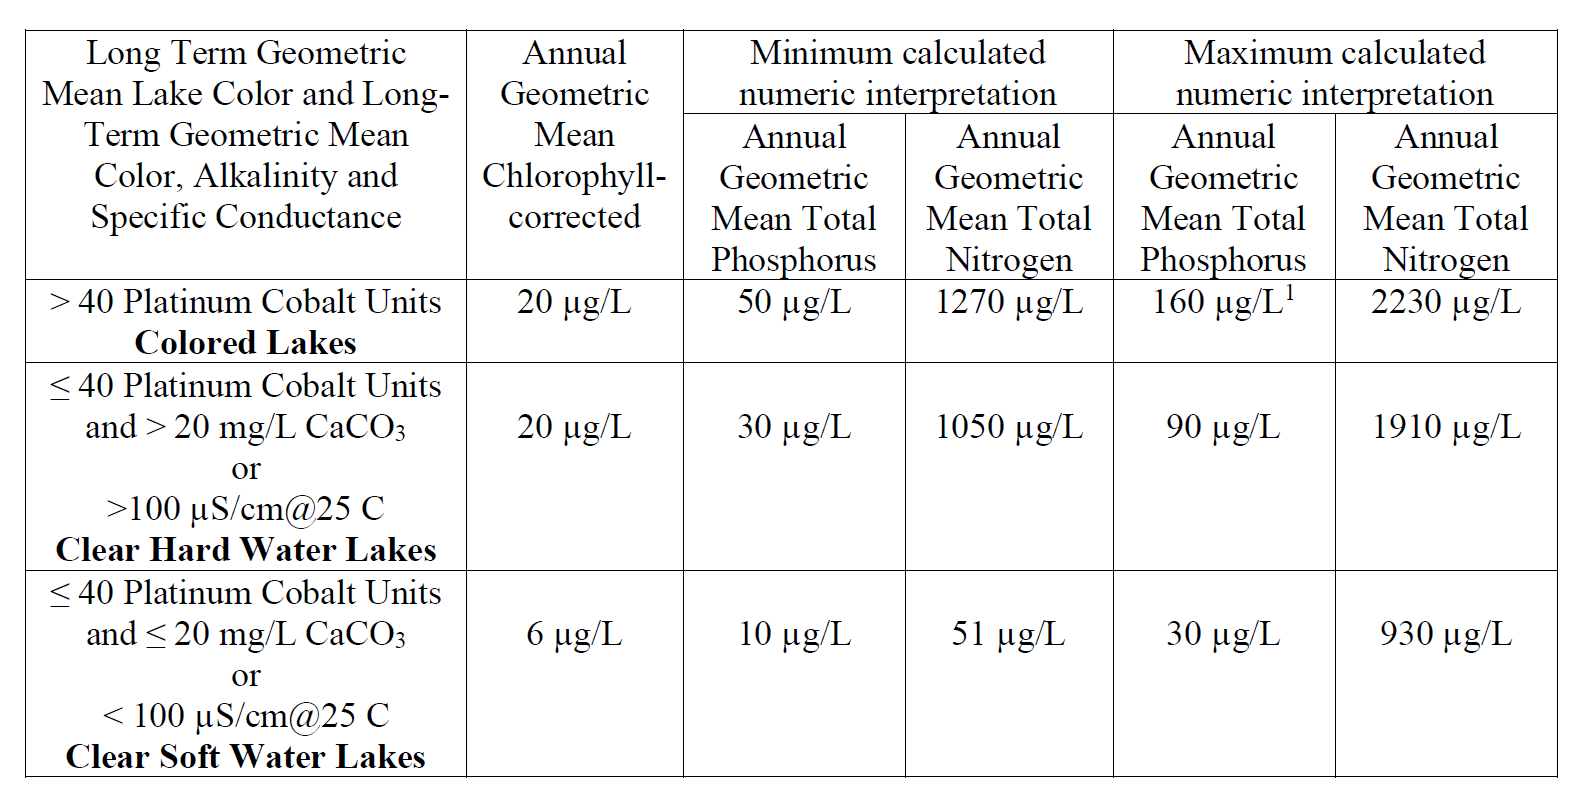
\includegraphics[width=21.97in]{LW Reports Table 1 V.2}

For the purpose of subparagraph 62-302.531(2)(b)1., F.A.C., color shall
be assessed as true color and shall be free from turbidity. Lake color
and alkalinity shall be the long-term geometric mean, based on a minimum
of ten data points over at least three years with at least one data
point in each year. If insufficient alkalinity data are available,
long-term geometric mean specific conductance values shall be used, with
a value of \textless100 µS/cm@25 C used to estimate the mg/L
CaCO\textsubscript{3} alkalinity concentration until such time that
alkalinity data are available.

\begin{Shaded}
\begin{Highlighting}[]
\NormalTok{knitr}\SpecialCharTok{::}\FunctionTok{include\_graphics}\NormalTok{(}\StringTok{"output/output\_table/table\_2.png"}\NormalTok{)}
\end{Highlighting}
\end{Shaded}

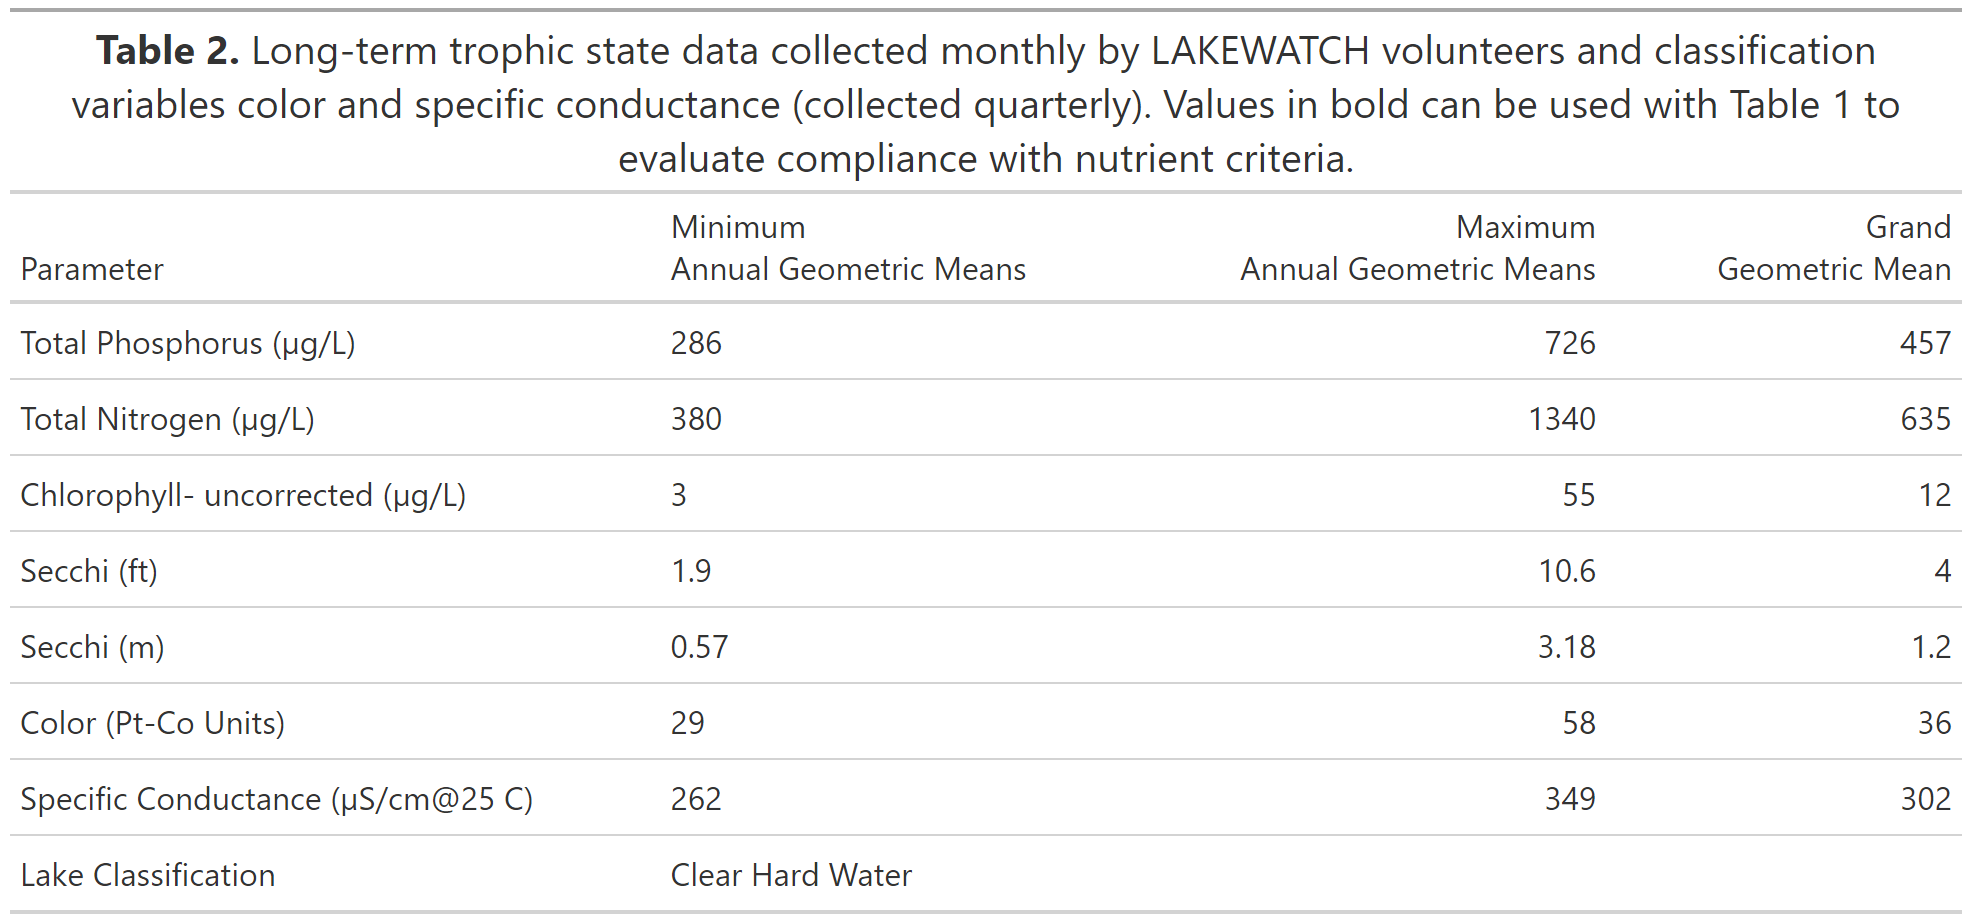
\includegraphics[width=27.39in]{output/output_table/table_2}

\hypertarget{table-3.-base-file-data-long-term-nutrient-grand-geometric-means-and-nutrient-zone-classification-listing-the-90th-percentile-concentrations-in-figure-1.-values-in-bold-can-be-used-for-nutrient-zone-comparisons.}{%
\subsubsection{Table 3. Base File Data, long-term nutrient grand
geometric means and Nutrient Zone classification listing the 90th
percentile concentrations in Figure 1. Values in bold can be used for
Nutrient Zone
comparisons.}\label{table-3.-base-file-data-long-term-nutrient-grand-geometric-means-and-nutrient-zone-classification-listing-the-90th-percentile-concentrations-in-figure-1.-values-in-bold-can-be-used-for-nutrient-zone-comparisons.}}

\#graph example

this is an example of the phosphorous graph, work in progress still

Figure 2 and Figure 3. Trend plots of annual average total phosphorus
and annual average total nitrogen versus year. The R2 value indicates
the strength of the relations (ranges from 0.0 to 1.0; higher the R2 the
stronger the relation) and the p value indicates if the relation is
significant (p \textless{} 0.05 is significant). Trend Status are
reported on plots.

\begin{Shaded}
\begin{Highlighting}[]
\CommentTok{\#lm for graph to refer to }

\NormalTok{total\_p\_lm }\OtherTok{=} \FunctionTok{lm}\NormalTok{(TP }\SpecialCharTok{\textasciitilde{}}\NormalTok{ Year, }\AttributeTok{data =}\NormalTok{ lake)}

\NormalTok{total\_p\_table }\OtherTok{=} \FunctionTok{glance}\NormalTok{(total\_p\_lm)}

\NormalTok{trend }\OtherTok{=} \FunctionTok{if\_else}\NormalTok{(total\_p\_table}\SpecialCharTok{$}\NormalTok{p.value }\SpecialCharTok{\textgreater{}=} \FloatTok{0.5}\NormalTok{, }\AttributeTok{true =} \StringTok{"No trend"}\NormalTok{, }\AttributeTok{false =} \FunctionTok{if\_else}\NormalTok{(total\_p\_lm[[}\StringTok{"coefficients"}\NormalTok{]][[}\StringTok{"Year"}\NormalTok{]] }\SpecialCharTok{\textgreater{}} \DecValTok{0}\NormalTok{ , }\AttributeTok{true =} \StringTok{"Increasing"}\NormalTok{, }\AttributeTok{false =} \StringTok{"Decreasing"}\NormalTok{))}
  
\NormalTok{plot\_title }\OtherTok{=} \FunctionTok{glue}\NormalTok{(}\StringTok{"Total Phosphorus (µg/L) by Year for Lake \{lake$Lake[1]\} in \{lake$County[1]\} County"}\NormalTok{)  }
  

\NormalTok{label }\OtherTok{=}\NormalTok{ (}\FunctionTok{glue}\NormalTok{(}\StringTok{"p = \{signif(total\_p\_table$p.value, digits = 2)\}, R\textless{}sup\textgreater{}2\textless{}/sup\textgreater{} = \{signif(total\_p\_table$r.squared, digits = 2)\}, \{trend\} "}\NormalTok{))}

\NormalTok{maxlim }\OtherTok{=} \FunctionTok{max}\NormalTok{(lake}\SpecialCharTok{$}\NormalTok{TP)}\SpecialCharTok{+}\DecValTok{10}
\NormalTok{minlim }\OtherTok{=} \FunctionTok{min}\NormalTok{(lake}\SpecialCharTok{$}\NormalTok{TP)}

\NormalTok{total\_p\_graph }\OtherTok{=} \FunctionTok{ggplot}\NormalTok{(}\AttributeTok{data =}\NormalTok{ lake, }\FunctionTok{aes}\NormalTok{(}\AttributeTok{x =}\NormalTok{ Year, }\AttributeTok{y =}\NormalTok{ TP)) }\SpecialCharTok{+}
  \FunctionTok{geom\_point}\NormalTok{() }\SpecialCharTok{+}
  \FunctionTok{geom\_smooth}\NormalTok{(}
    \AttributeTok{method =} \StringTok{"lm"}\NormalTok{, }
    \AttributeTok{se =} \ConstantTok{FALSE}\NormalTok{, }
    \AttributeTok{linetype =} \FunctionTok{paste}\NormalTok{(}
      \FunctionTok{if\_else}\NormalTok{(total\_p\_table}\SpecialCharTok{$}\NormalTok{p.value }\SpecialCharTok{\textless{}=} \FloatTok{0.5}\NormalTok{,}\AttributeTok{true =} \StringTok{"solid"}\NormalTok{, }\AttributeTok{false =} \StringTok{"dashed"}\NormalTok{ )}
\NormalTok{      )}
\NormalTok{    ) }\SpecialCharTok{+}
  \FunctionTok{labs}\NormalTok{(}\AttributeTok{title =}\NormalTok{ plot\_title, }\AttributeTok{x =} \StringTok{"Year"}\NormalTok{, }\AttributeTok{y =} \StringTok{"Total Phosphorus (µg/L)"}\NormalTok{)}\SpecialCharTok{+}
  \FunctionTok{theme\_bw}\NormalTok{() }\SpecialCharTok{+}
  \FunctionTok{theme}\NormalTok{(}\AttributeTok{plot.title =} \FunctionTok{element\_text}\NormalTok{(}\AttributeTok{hjust =} \FloatTok{0.5}\NormalTok{)) }\SpecialCharTok{+} \FunctionTok{geom\_richtext}\NormalTok{(}
    \AttributeTok{label =}\NormalTok{ label}
\NormalTok{    ,}\AttributeTok{x =}\NormalTok{ (}\FunctionTok{min}\NormalTok{(lake}\SpecialCharTok{$}\NormalTok{Year, }\AttributeTok{na.rm =} \ConstantTok{TRUE}\NormalTok{)}\SpecialCharTok{+}\DecValTok{5}\NormalTok{),}
    \AttributeTok{y =}\NormalTok{ (}\FunctionTok{max}\NormalTok{(lake}\SpecialCharTok{$}\NormalTok{TP, }\AttributeTok{na.rm =} \ConstantTok{TRUE}\NormalTok{)}\SpecialCharTok{+}\DecValTok{5}\NormalTok{),}
\NormalTok{    )}\SpecialCharTok{+}\FunctionTok{ylim}\NormalTok{(minlim, maxlim)}


\FunctionTok{show}\NormalTok{(total\_p\_graph)}
\end{Highlighting}
\end{Shaded}

\begin{verbatim}
## `geom_smooth()` using formula = 'y ~ x'
\end{verbatim}

\includegraphics{LWReport-Markdown-Code_files/figure-latex/p_graph-1.pdf}

\begin{Shaded}
\begin{Highlighting}[]
\NormalTok{total\_n\_lm }\OtherTok{=} \FunctionTok{lm}\NormalTok{(TN }\SpecialCharTok{\textasciitilde{}}\NormalTok{ Year, }\AttributeTok{data =}\NormalTok{ lake)}

\NormalTok{total\_n\_table }\OtherTok{=} \FunctionTok{glance}\NormalTok{(total\_n\_lm)}

\NormalTok{trend }\OtherTok{=} \FunctionTok{if\_else}\NormalTok{(total\_n\_table}\SpecialCharTok{$}\NormalTok{p.value }\SpecialCharTok{\textgreater{}=} \FloatTok{0.5}\NormalTok{, }\AttributeTok{true =} \StringTok{"No trend"}\NormalTok{, }\AttributeTok{false =} \FunctionTok{if\_else}\NormalTok{(total\_n\_lm[[}\StringTok{"coefficients"}\NormalTok{]][[}\StringTok{"Year"}\NormalTok{]] }\SpecialCharTok{\textgreater{}} \DecValTok{0}\NormalTok{ , }\AttributeTok{true =} \StringTok{"Increasing"}\NormalTok{, }\AttributeTok{false =} \StringTok{"Decreasing"}\NormalTok{))}
  
\NormalTok{plot\_title }\OtherTok{=} \FunctionTok{glue}\NormalTok{(}\StringTok{"Total Nitrogen (µg/L) by Year for Lake \{lake$Lake[1]\} in \{lake$County[1]\} County"}\NormalTok{)  }
  

\NormalTok{label }\OtherTok{=}\NormalTok{ (}\FunctionTok{glue}\NormalTok{(}\StringTok{"p = \{signif(total\_n\_table$p.value, digits = 2)\}, R\textless{}sup\textgreater{}2\textless{}/sup\textgreater{} = \{signif(total\_n\_table$r.squared, digits = 2)\}, \{trend\} "}\NormalTok{))}

\NormalTok{maxlim }\OtherTok{=} \FunctionTok{max}\NormalTok{(lake}\SpecialCharTok{$}\NormalTok{TN)}\SpecialCharTok{+}\DecValTok{10}
\NormalTok{minlim }\OtherTok{=} \FunctionTok{min}\NormalTok{(lake}\SpecialCharTok{$}\NormalTok{TN)}

\NormalTok{total\_n\_graph }\OtherTok{=} \FunctionTok{ggplot}\NormalTok{(}\AttributeTok{data =}\NormalTok{ lake, }\FunctionTok{aes}\NormalTok{(}\AttributeTok{x =}\NormalTok{ Year, }\AttributeTok{y =}\NormalTok{ TN)) }\SpecialCharTok{+}
  \FunctionTok{geom\_point}\NormalTok{() }\SpecialCharTok{+}
  \FunctionTok{geom\_smooth}\NormalTok{(}
    \AttributeTok{method =} \StringTok{"lm"}\NormalTok{, }
    \AttributeTok{se =} \ConstantTok{FALSE}\NormalTok{, }
    \AttributeTok{linetype =} \FunctionTok{paste}\NormalTok{(}
      \FunctionTok{if\_else}\NormalTok{(total\_n\_table}\SpecialCharTok{$}\NormalTok{p.value }\SpecialCharTok{\textless{}=} \FloatTok{0.5}\NormalTok{,}\AttributeTok{true =} \StringTok{"solid"}\NormalTok{, }\AttributeTok{false =} \StringTok{"dashed"}\NormalTok{ )}
\NormalTok{      )}
\NormalTok{    ) }\SpecialCharTok{+}
  \FunctionTok{labs}\NormalTok{(}\AttributeTok{title =}\NormalTok{ plot\_title, }\AttributeTok{x =} \StringTok{"Year"}\NormalTok{, }\AttributeTok{y =} \StringTok{"Total Nitrogen (µg/L)"}\NormalTok{)}\SpecialCharTok{+}
  \FunctionTok{theme\_bw}\NormalTok{() }\SpecialCharTok{+}
  \FunctionTok{theme}\NormalTok{(}\AttributeTok{plot.title =} \FunctionTok{element\_text}\NormalTok{(}\AttributeTok{hjust =} \FloatTok{0.5}\NormalTok{)) }\SpecialCharTok{+} \FunctionTok{geom\_richtext}\NormalTok{(}
    \AttributeTok{label =}\NormalTok{ label}
\NormalTok{    ,}\AttributeTok{x =}\NormalTok{ (}\FunctionTok{min}\NormalTok{(lake}\SpecialCharTok{$}\NormalTok{Year, }\AttributeTok{na.rm =} \ConstantTok{TRUE}\NormalTok{)}\SpecialCharTok{+}\DecValTok{5}\NormalTok{),}
    \AttributeTok{y =}\NormalTok{ (}\FunctionTok{max}\NormalTok{(lake}\SpecialCharTok{$}\NormalTok{TN, }\AttributeTok{na.rm =} \ConstantTok{TRUE}\NormalTok{)}\SpecialCharTok{+}\DecValTok{5}\NormalTok{),}
\NormalTok{    )}\SpecialCharTok{+}\FunctionTok{ylim}\NormalTok{(minlim, maxlim)}


\FunctionTok{show}\NormalTok{(total\_n\_graph)}
\end{Highlighting}
\end{Shaded}

\begin{verbatim}
## `geom_smooth()` using formula = 'y ~ x'
\end{verbatim}

\includegraphics{LWReport-Markdown-Code_files/figure-latex/n_graph-1.pdf}

Figure 4 and Figure 5. Trend plots of annual average chlorophyll and
annual average Secchi versus year. The R2 value indicates the strength
of the relations (ranges from 0.0 to 1.0; higher the R2 the stronger the
relations and the p value indicates if the relation is significant (p
\textless{} 0.05 is significant). Trend status are reported on plots.

\begin{Shaded}
\begin{Highlighting}[]
\NormalTok{total\_chl\_lm }\OtherTok{=} \FunctionTok{lm}\NormalTok{(CHL }\SpecialCharTok{\textasciitilde{}}\NormalTok{ Year, }\AttributeTok{data =}\NormalTok{ lake)}

\NormalTok{total\_chl\_table }\OtherTok{=} \FunctionTok{glance}\NormalTok{(total\_chl\_lm)}

\NormalTok{trend }\OtherTok{=} \FunctionTok{if\_else}\NormalTok{(total\_chl\_table}\SpecialCharTok{$}\NormalTok{p.value }\SpecialCharTok{\textgreater{}=} \FloatTok{0.5}\NormalTok{, }\AttributeTok{true =} \StringTok{"No trend"}\NormalTok{, }\AttributeTok{false =} \FunctionTok{if\_else}\NormalTok{(total\_chl\_lm[[}\StringTok{"coefficients"}\NormalTok{]][[}\StringTok{"Year"}\NormalTok{]] }\SpecialCharTok{\textgreater{}} \DecValTok{0}\NormalTok{ , }\AttributeTok{true =} \StringTok{"Increasing"}\NormalTok{, }\AttributeTok{false =} \StringTok{"Decreasing"}\NormalTok{))}
  
\NormalTok{plot\_title }\OtherTok{=} \FunctionTok{glue}\NormalTok{(}\StringTok{"Total Chlorophyll (µg/L) by Year for Lake \{lake$Lake[1]\} in \{lake$County[1]\} County"}\NormalTok{)  }
  

\NormalTok{label }\OtherTok{=}\NormalTok{ (}\FunctionTok{glue}\NormalTok{(}\StringTok{"p = \{signif(total\_chl\_table$p.value, digits = 2)\}, R\textless{}sup\textgreater{}2\textless{}/sup\textgreater{} = \{signif(total\_chl\_table$r.squared, digits = 2)\}, \{trend\} "}\NormalTok{))}

\NormalTok{maxlim }\OtherTok{=} \FunctionTok{max}\NormalTok{(lake}\SpecialCharTok{$}\NormalTok{CHL)}\SpecialCharTok{+}\DecValTok{10}
\NormalTok{minlim }\OtherTok{=} \FunctionTok{min}\NormalTok{(lake}\SpecialCharTok{$}\NormalTok{CHL)}

\NormalTok{total\_chl\_graph }\OtherTok{=} \FunctionTok{ggplot}\NormalTok{(}\AttributeTok{data =}\NormalTok{ lake, }\FunctionTok{aes}\NormalTok{(}\AttributeTok{x =}\NormalTok{ Year, }\AttributeTok{y =}\NormalTok{ CHL)) }\SpecialCharTok{+}
  \FunctionTok{geom\_point}\NormalTok{() }\SpecialCharTok{+}
  \FunctionTok{geom\_smooth}\NormalTok{(}
    \AttributeTok{method =} \StringTok{"lm"}\NormalTok{, }
    \AttributeTok{se =} \ConstantTok{FALSE}\NormalTok{, }
    \AttributeTok{linetype =} \FunctionTok{paste}\NormalTok{(}
      \FunctionTok{if\_else}\NormalTok{(total\_chl\_table}\SpecialCharTok{$}\NormalTok{p.value }\SpecialCharTok{\textless{}=} \FloatTok{0.5}\NormalTok{,}\AttributeTok{true =} \StringTok{"solid"}\NormalTok{, }\AttributeTok{false =} \StringTok{"dashed"}\NormalTok{ )}
\NormalTok{      )}
\NormalTok{    ) }\SpecialCharTok{+}
  \FunctionTok{labs}\NormalTok{(}\AttributeTok{title =}\NormalTok{ plot\_title, }\AttributeTok{x =} \StringTok{"Year"}\NormalTok{, }\AttributeTok{y =} \StringTok{"Total Chlorophyll (µg/L)"}\NormalTok{)}\SpecialCharTok{+}
  \FunctionTok{theme\_bw}\NormalTok{() }\SpecialCharTok{+}
  \FunctionTok{theme}\NormalTok{(}\AttributeTok{plot.title =} \FunctionTok{element\_text}\NormalTok{(}\AttributeTok{hjust =} \FloatTok{0.5}\NormalTok{)) }\SpecialCharTok{+} \FunctionTok{geom\_richtext}\NormalTok{(}
    \AttributeTok{label =}\NormalTok{ label}
\NormalTok{    ,}\AttributeTok{x =}\NormalTok{ (}\FunctionTok{min}\NormalTok{(lake}\SpecialCharTok{$}\NormalTok{Year,}\AttributeTok{na.rm =} \ConstantTok{TRUE}\NormalTok{)}\SpecialCharTok{+}\DecValTok{5}\NormalTok{),}
    \AttributeTok{y =}\NormalTok{ (}\FunctionTok{max}\NormalTok{(lake}\SpecialCharTok{$}\NormalTok{CHL, }\AttributeTok{na.rm =} \ConstantTok{TRUE}\NormalTok{)}\SpecialCharTok{+}\DecValTok{5}\NormalTok{),}
\NormalTok{    )}\SpecialCharTok{+}\FunctionTok{ylim}\NormalTok{(minlim, maxlim)}

\FunctionTok{show}\NormalTok{(total\_chl\_graph)}
\end{Highlighting}
\end{Shaded}

\begin{verbatim}
## `geom_smooth()` using formula = 'y ~ x'
\end{verbatim}

\includegraphics{LWReport-Markdown-Code_files/figure-latex/chl_graph-1.pdf}

\begin{Shaded}
\begin{Highlighting}[]
\NormalTok{total\_secchi\_lm }\OtherTok{=} \FunctionTok{lm}\NormalTok{(SECCHI\_ft }\SpecialCharTok{\textasciitilde{}}\NormalTok{ Year, }\AttributeTok{data =}\NormalTok{ lake)}

\NormalTok{total\_secchi\_table }\OtherTok{=} \FunctionTok{glance}\NormalTok{(total\_secchi\_lm)}

\NormalTok{trend }\OtherTok{=} \FunctionTok{if\_else}\NormalTok{(total\_secchi\_table}\SpecialCharTok{$}\NormalTok{p.value }\SpecialCharTok{\textgreater{}=} \FloatTok{0.5}\NormalTok{, }\AttributeTok{true =} \StringTok{"No trend"}\NormalTok{, }\AttributeTok{false =} \FunctionTok{if\_else}\NormalTok{(total\_secchi\_lm[[}\StringTok{"coefficients"}\NormalTok{]][[}\StringTok{"Year"}\NormalTok{]] }\SpecialCharTok{\textgreater{}} \DecValTok{0}\NormalTok{ , }\AttributeTok{true =} \StringTok{"Increasing"}\NormalTok{, }\AttributeTok{false =} \StringTok{"Decreasing"}\NormalTok{))}
  
\NormalTok{plot\_title }\OtherTok{=} \FunctionTok{glue}\NormalTok{(}\StringTok{"Secchi Depth (ft) by Year for Lake \{lake$Lake[1]\} in \{lake$County[1]\} County"}\NormalTok{)  }
  

\NormalTok{label }\OtherTok{=}\NormalTok{ (}\FunctionTok{glue}\NormalTok{(}\StringTok{"p = \{signif(total\_secchi\_table$p.value, digits = 2)\}, R\textless{}sup\textgreater{}2\textless{}/sup\textgreater{} = \{signif(total\_secchi\_table$r.squared, digits = 2)\}, \{trend\} "}\NormalTok{))}

\NormalTok{maxlim }\OtherTok{=} \FunctionTok{max}\NormalTok{(lake}\SpecialCharTok{$}\NormalTok{SECCHI\_ft, }\AttributeTok{na.rm =} \ConstantTok{TRUE}\NormalTok{)}\SpecialCharTok{+}\DecValTok{10}
\NormalTok{minlim }\OtherTok{=} \FunctionTok{min}\NormalTok{(lake}\SpecialCharTok{$}\NormalTok{SECCHI\_ft, }\AttributeTok{na.rm =} \ConstantTok{TRUE}\NormalTok{)}

\NormalTok{total\_secchi\_graph }\OtherTok{=} \FunctionTok{ggplot}\NormalTok{(}\AttributeTok{data =}\NormalTok{ lake, }\FunctionTok{aes}\NormalTok{(}\AttributeTok{x =}\NormalTok{ Year, }\AttributeTok{y =}\NormalTok{ SECCHI\_ft)) }\SpecialCharTok{+}
  \FunctionTok{geom\_point}\NormalTok{() }\SpecialCharTok{+}
  \FunctionTok{geom\_smooth}\NormalTok{(}
    \AttributeTok{method =} \StringTok{"lm"}\NormalTok{, }
    \AttributeTok{se =} \ConstantTok{FALSE}\NormalTok{, }
    \AttributeTok{linetype =} \FunctionTok{paste}\NormalTok{(}
      \FunctionTok{if\_else}\NormalTok{(total\_secchi\_table}\SpecialCharTok{$}\NormalTok{p.value }\SpecialCharTok{\textless{}=} \FloatTok{0.5}\NormalTok{,}\AttributeTok{true =} \StringTok{"solid"}\NormalTok{, }\AttributeTok{false =} \StringTok{"dashed"}\NormalTok{ )}
\NormalTok{      )}
\NormalTok{    ) }\SpecialCharTok{+}
  \FunctionTok{labs}\NormalTok{(}\AttributeTok{title =}\NormalTok{ plot\_title, }\AttributeTok{x =} \StringTok{"Year"}\NormalTok{, }\AttributeTok{y =} \StringTok{"Secchi depth (ft)"}\NormalTok{)}\SpecialCharTok{+}
  \FunctionTok{theme\_bw}\NormalTok{() }\SpecialCharTok{+}
  \FunctionTok{theme}\NormalTok{(}\AttributeTok{plot.title =} \FunctionTok{element\_text}\NormalTok{(}\AttributeTok{hjust =} \FloatTok{0.5}\NormalTok{)) }\SpecialCharTok{+} \FunctionTok{geom\_richtext}\NormalTok{(}
    \AttributeTok{label =}\NormalTok{ label,}
    \AttributeTok{x =}\NormalTok{ (}\FunctionTok{min}\NormalTok{(lake}\SpecialCharTok{$}\NormalTok{Year, }\AttributeTok{na.rm =} \ConstantTok{TRUE}\NormalTok{)}\SpecialCharTok{+}\DecValTok{5}\NormalTok{),}
    \AttributeTok{y =}\NormalTok{ (}\FunctionTok{max}\NormalTok{(lake}\SpecialCharTok{$}\NormalTok{SECCHI\_ft, }\AttributeTok{na.rm =} \ConstantTok{TRUE}\NormalTok{)}\SpecialCharTok{+}\DecValTok{5}\NormalTok{)}
\NormalTok{    )}\SpecialCharTok{+}\FunctionTok{ylim}\NormalTok{(minlim, maxlim)}
  



\FunctionTok{show}\NormalTok{(total\_secchi\_graph)}
\end{Highlighting}
\end{Shaded}

\begin{verbatim}
## `geom_smooth()` using formula = 'y ~ x'
\end{verbatim}

\begin{verbatim}
## Warning: Removed 22 rows containing non-finite values (`stat_smooth()`).
\end{verbatim}

\begin{verbatim}
## Warning: Removed 22 rows containing missing values (`geom_point()`).
\end{verbatim}

\includegraphics{LWReport-Markdown-Code_files/figure-latex/secchi_graph-1.pdf}

\end{document}
